\section{Where is the meaning?}



\begin{frame}{Referential or Representational?}

One view of meaning is to define it in terms of how it constrains reality.

\begin{itemize}
\item Picture the worlds in which these sentences are true:
  \begin{exe}
    \ex \eng{I patted the dog.}
    \ex \eng{I did not pat the dog.}
  \end{exe}
\end{itemize}

Assuming that they were uttered at the same time, they are
incompatible because they cannot refer to the same
situation: the \txx{referential} view. 
\newpage
But we can represent the same reality in different ways:

\begin{exe}
  \ex \eng{Ich habe Hunger} ``I have hunger''
  \ex \eng{I am hungry}
\end{exe}

\txx{Representational} theories are interested in how we represent reality,
and how our representations are influenced by conceptual structures
conventionalized in language.


 \end{frame}

\begin{frame}{Referential View}

\begin{center}
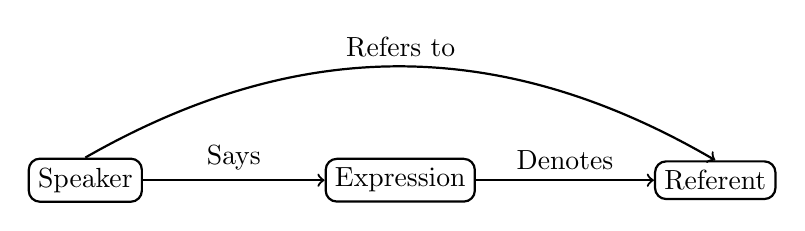
\begin{tikzpicture}[node distance=4cm, auto, thick]
  \node[draw, rounded corners](speaker){Speaker};
  \node[draw, rounded corners, right of=speaker](expression){Expression};
  \node[draw, rounded corners, right of=expression](referent){Referent};

  \draw[->, thick] (speaker) -- node{Says}(expression);
  \draw[->, thick] (expression) -- node{Denotes}(referent);
  \draw[->, thick, bend left] (speaker.north) to node[above]{Refers to}(referent.north);
\end{tikzpicture}
\end{center}


 The \txx{referential view} is focused on direct relationships between
 expressions (words, sentences) and things in the world (realist
 view).

 \end{frame}

\begin{frame}{Representational View}

\begin{center}
\begin{tikzpicture}[node distance=4cm, auto, thick]
  \node[draw, rounded corners](speaker){Speaker};
  \node[draw, rounded corners, right of=speaker](expression){Expression};
  \node[draw, rounded corners, above right=of expression, xshift=-4cm, yshift=0cm] (concept) {Concept};
  \node[draw, rounded corners, right=of expression, xshift=-2cm] (referent) {Referent};

  \draw[->, thick] (speaker) -- node{Says}(expression);
  \draw[->, thick] (expression) -- node{Evokes}(concept);
  \draw[->, thick] (concept) -- node[right]{Represents/Refers-to}(referent);
  \draw[->, thick] (speaker) to node[left]{Refers via}(concept);
\end{tikzpicture}
\end{center}

 The \txx{representational view} is focused on how relationships between
 expressions (words, sentences) and things in the world are mediated by
 the mind (cognitive linguistics).  

This gives a more complex, but richer model.


\end{frame}

\begin{frame}{Referring vs Non-Referring}

\begin{itemize}
\item \txx{Referring expressions} are expressions that identify
  entities in the world (typically \txx{nominals})
  \begin{exe}
    \ex \eng{cat}, \jpn[that yellow bag]{ano kiiro kaban}
    \ex \eng{London Bridge}, \eng{Xiao Ming}
  \end{exe}
\item \txx{Non-referring expressions} don't have referential properties
  \begin{exe}
    \ex \eng{maybe, if, is, but}
  \end{exe}
\item Not all nominals refer
  \begin{exe}
    \ex \eng{That is \ul{an ugly dog}}
    \ex \eng{If only I had \ul{a dog}}
  \end{exe}
\item And, of course, all this is made more confusing if we model the
  fictional world and our interpretation of it as separate from the
  characters' interpretations, \ldots
\end{itemize}
\end{frame}



\begin{frame}{Further Reading}

\begin{itemize}
\item Introduction What does it mean to mean?
  \begin{itemize}
  \item Saeed: \S~2
  \end{itemize}
\end{itemize}
\end{frame}



